\documentclass[aspectratio=169]{beamer}

\geometry{mag=1587,truedimen}

% pdftk A=hasco_2022.pdf B=2022\ ROOT\ Summer\ Student\ Course.pdf cat A1-16 B32 A17-18 B35-36 A20-28 B55-62 B64-64 A38-52 B87-94 B96-97 A62-68 output ROOT_HASCO_2022.pdf

%
% Choose how your presentation looks.
%
% For more themes, color themes and font themes, see:
% http://deic.uab.es/~iblanes/beamer_gallery/index_by_theme.html
%
\mode<presentation>
{
  \usetheme{default}      % or try Darmstadt, Madrid, Warsaw, ...
  \usecolortheme{default} % or try albatross, beaver, crane, ...
  \usefonttheme{default}  % or try serif, structurebold, ...
  \setbeamertemplate{navigation symbols}{}
  \setbeamertemplate{caption}[numbered]
}

\AtBeginSection[]{
  \begin{frame}
  \vfill
  \centering
  \begin{beamercolorbox}[sep=8pt,center,shadow=true,rounded=true]{title}
    \usebeamerfont{title}\insertsectionhead\par%
  \end{beamercolorbox}
  \vfill
  \end{frame}
}

\usepackage[english]{babel}
\usepackage[utf8]{inputenc}
\usepackage[T1]{fontenc}
%\usepackage{inconsolata} % to get a nice monospace font for code listings
\usepackage[scaled]{beramono}
\usepackage[most]{tcolorbox}
\usepackage{listings}
\usepackage{hyperref,xcolor}% http://ctan.org/pkg/{hyperref,xcolor}
\usepackage{colortbl}
\usepackage{tikz}
\usetikzlibrary{arrows.meta}


\setbeamertemplate
%{footline}{\quad\hfill\insertframenumber/\inserttotalframenumber\strut\quad~}
{footline}{\quad\hfill\insertframenumber\strut\quad~}

\definecolor{myblue}{RGB}{51,51,178}
\definecolor{darkgreen}{RGB}{51,178,51}

\hypersetup
{
    pdfauthor={Jonas Rembser},
    pdfsubject={ROOT Lecture},
    pdftitle={ROOT Lecture},
    pdfkeywords={ROOT}
%    colorlinks=false,
    %pdfborder={0 0 0},
%You can set individual colors for links as below:
%colorlinks=true,
%linkcolor=myblue,
%urlcolor={myblue},
%filecolor={myblue},
%citecolor={myblue},
%allcolors={myblue}
}

%%%%%%%%%%%%%%%%%%%%

\definecolor{white}{rgb}{1,1,1}
\definecolor{mygreen}{rgb}{0,0.4,0}
\definecolor{light_gray}{rgb}{0.97,0.97,0.97}
\definecolor{mykey}{rgb}{0.117,0.403,0.713}

\tcbuselibrary{listings}
\newlength\inwd
\setlength\inwd{1.3cm}

\newcounter{ipythcntr}
\renewcommand{\theipythcntr}{\texttt{[\arabic{ipythcntr}]}}

\newtcblisting{cppcell}[1][]{%
  sharp corners,
  %enlarge left by=\inwd,
  %width=\linewidth-\inwd,
  width=\linewidth,
  enhanced,
  boxrule=0pt,
  colback=light_gray,
  listing only,
  top=0pt,
  bottom=0pt,
  overlay={
    %\node[
      %anchor=north east,
      %text width=\inwd,
      %font=\footnotesize\ttfamily\color{mykey},
      %inner ysep=2mm,
      %inner xsep=0pt,
      %outer sep=0pt
      %]
      %at (frame.north west)
      %{\refstepcounter{ipythcntr}\label{#1}In \theipythcntr:};
  }
  listing engine=listing,
  listing options={
    aboveskip=1pt,
    belowskip=1pt,
    basicstyle=\footnotesize\ttfamily,
    language=C++,
    keywordstyle=\color{mykey},
    showstringspaces=false,
    stringstyle=\color{mygreen}
  },
}

\newtcblisting{pycell}[1][]{%
  sharp corners,
  %enlarge left by=\inwd,
  %width=\linewidth-\inwd,
  width=\linewidth,
  enhanced,
  boxrule=0pt,
  colback=light_gray,
  listing only,
  top=0pt,
  bottom=0pt,
  overlay={
    %\node[
      %anchor=north east,
      %text width=\inwd,
      %font=\footnotesize\ttfamily\color{mykey},
      %inner ysep=2mm,
      %inner xsep=0pt,
      %outer sep=0pt
      %]
      %at (frame.north west)
      %{\refstepcounter{ipythcntr}\label{#1}In \theipythcntr:};
  }
  listing engine=listing,
  listing options={
    aboveskip=1pt,
    belowskip=1pt,
    basicstyle=\footnotesize\ttfamily,
    language=Python,
    keywordstyle=\color{mykey},
    showstringspaces=false,
    stringstyle=\color{mygreen}
  },
}

\newtcblisting{pycelltiny}[1][]{%
  sharp corners,
  %enlarge left by=\inwd,
  %width=\linewidth-\inwd,
  width=\linewidth,
  enhanced,
  boxrule=0pt,
  colback=light_gray,
  listing only,
  top=0pt,
  bottom=0pt,
  overlay={
    %\node[
      %anchor=north east,
      %text width=\inwd,
      %font=\footnotesize\ttfamily\color{mykey},
      %inner ysep=2mm,
      %inner xsep=0pt,
      %outer sep=0pt
      %]
      %at (frame.north west)
      %{\refstepcounter{ipythcntr}\label{#1}In \theipythcntr:};
  }
  listing engine=listing,
  listing options={
    aboveskip=1pt,
    belowskip=1pt,
    basicstyle=\tiny\ttfamily,
    language=Python,
    keywordstyle=\color{mykey},
    showstringspaces=false,
    stringstyle=\color{mygreen}
  },
}
\newtcblisting{cellprint}{
  sharp corners,
  enlarge left by=\inwd,
  width=\linewidth-\inwd,
  enhanced,
  boxrule=0pt,
  colback=white,
  listing only,
  top=0pt,
  bottom=0pt,
  overlay={
    \node[
      anchor=north east,
      text width=\inwd,
      font=\footnotesize\ttfamily\color{mykey},
      inner ysep=2mm,
      inner xsep=0pt,
      outer sep=0pt
      ]
      at (frame.north west)
      {};
  }
  listing engine=listing,
  listing options={
      aboveskip=1pt,
      belowskip=1pt,
      basicstyle=\footnotesize\ttfamily,
      language=Python,
      keywordstyle=\color{mykey},
      showstringspaces=false,
      stringstyle=\color{mygreen}
    },
}
\newtcblisting{cellout}[1][\theipythcntr]{
  sharp corners,
  enlarge left by=\inwd,
  width=\linewidth-\inwd,
  enhanced,
  boxrule=0pt,
  colback=white,
  listing only,
  top=0pt,
  bottom=0pt,
  overlay={
    \node[
      anchor=north east,
      text width=\inwd,
      font=\footnotesize\ttfamily\color{mykey},
      inner ysep=2mm,
      inner xsep=0pt,
      outer sep=0pt
      ]
      at (frame.north west)
      {\setcounter{ipythcntr}{\value{ipythcntr}}Out#1:};
  }
  listing engine=listing,
  listing options={
      aboveskip=1pt,
      belowskip=1pt,
      basicstyle=\footnotesize\ttfamily,
      language=Python,
      keywordstyle=\color{mykey},
      showstringspaces=false,
      stringstyle=\color{mygreen}
    },
}

%%%%%%%%%%%%%%%%%%%%

\definecolor{terminal-bg}{RGB}{63, 63, 63}
\definecolor{terminal-fg}{RGB}{220, 220, 204}
\definecolor{terminal-fg-emph}{RGB}{245, 180, 0}

\newcommand{\myterminalinline}[1]{
    \colorbox{terminal-bg}{{\color{terminal-fg}\texttt{#1}}}
}

\newcommand{\emphinlisting}[1]{{\color{terminal-fg-emph}\textbf{#1}}}
\newcommand{\emphlightinlisting}[1]{{\color{terminal-fg-emph}#1}}

\newtcblisting{myterminal}[1][\theipythcntr]{
  sharp corners,
  enhanced,
  boxrule=0pt,
  %boxsep=0pt,
  colback=terminal-bg,
  coltext=terminal-fg,
  listing only,
  top=0pt,
  bottom=0pt,
  overlay={}
  listing engine=listing,
  listing options={
      xleftmargin=-10pt,
      %framesep=1pt,
      aboveskip=1pt,
      belowskip=1pt,
      basicstyle=\footnotesize\ttfamily,
      %language=Python,
      keywordstyle=\color{mykey},
      showstringspaces=false,
      stringstyle=\color{mygreen}
    },
}

\newtcblisting{myterminaltiny}[1][\theipythcntr]{
  sharp corners,
  enhanced,
  boxrule=0pt,
  %boxsep=0pt,
  colback=terminal-bg,
  coltext=terminal-fg,
  listing only,
  top=0pt,
  bottom=0pt,
  overlay={}
  listing engine=listing,
  listing options={
      xleftmargin=-10pt,
      aboveskip=1pt,
      belowskip=1pt,
      basicstyle=\tiny\ttfamily,
      %language=Python,
      keywordstyle=\color{mykey},
      showstringspaces=false,
      stringstyle=\color{mygreen}
    },
}

\graphicspath{{figures/}} %Setting the graphicspath

\newcommand{\myfigure}[2]{
    \begin{figure}
        \makebox[\textwidth]{%
            \includegraphics[width=#1\textwidth]{#2}
        }
    \end{figure}
}

\newcommand{\myhref}[2]{{\color{blue}\href{#1}{\underline{#2}}}}


\title[Your Short Title]{ROOT Lecture}
\author{Jonas Rembser}
\institute{CERN (EP-SFT)}
\date{July 20, 2023}

\begin{document}

\begin{frame}
    \titlepage
\end{frame}

% Uncomment these lines for an automatically generated outline.
%\begin{frame}{Outline}
%  \tableofcontents
%\end{frame}

\begin{frame}{Acknowledgments}
    This lecture and slides was inspired by the following lectures in the past:
    \vspace{3mm}
    \begin{itemize}
        \item The \myhref{https://indico.cern.ch/event/704163/contributions/2936717/attachments/1690757/2720489/StevenSchramm-IntroROOT.pdf}{lecture} and \myhref{https://indico.cern.ch/event/704163/contributions/2936719/attachments/1693833/2727086/Tutorial-ROOT.pdf}{exercises} from the HASCO 2018 by Steven Schramm
        \item The \myhref{https://indico.cern.ch/event/999261/contributions/4197218/attachments/2285603/3884654/hasco_root_2021.pdf}{lecture} and \myhref{https://indico.cern.ch/event/999261/contributions/4197219/attachments/2285604/3884655/hasco_root_tutorial_2021.pdf}{exercises} from the HASCO 2021 by Antonio Sidoti
        \item \myhref{https://github.com/root-project/training/tree/master/SummerStudentCourse/2023}{The ROOT Summer Student Course} at CERN from 2023
    \end{itemize}
    \vspace{3mm}
    This year, we will also cover an additional {\color{red}new ROOT feature}: the \textbf{RDataFrame}.

    \vspace{6mm}

    About me:
    \vspace{3mm}
    \begin{itemize}
    \item I did a PhD working with the CMS collaboration, graduated in 2020
    \item Right after, I joined the ROOT team at CERN to work on support and development of the \textbf{RooFit} package
    \end{itemize}
\end{frame}

\section{Introduction}

\begin{frame}{Introduction}
\begin{itemize}
    \item \textbf{Analysis} and \textbf{visualization} are fundamental in particle physics (experimental and not only)
\item ROOT is the primary tool for data analysis in \textbf{high energy physics} (not only collider physics)
\item Maybe not the reference tool if you are doing detector R\&D, theory/phenomenology, machine learning $\Rightarrow$ Useful to have an idea on how to use it since at some point you will use it
\end{itemize}
\end{frame}

\begin{frame}{History}
    \begin{figure}
        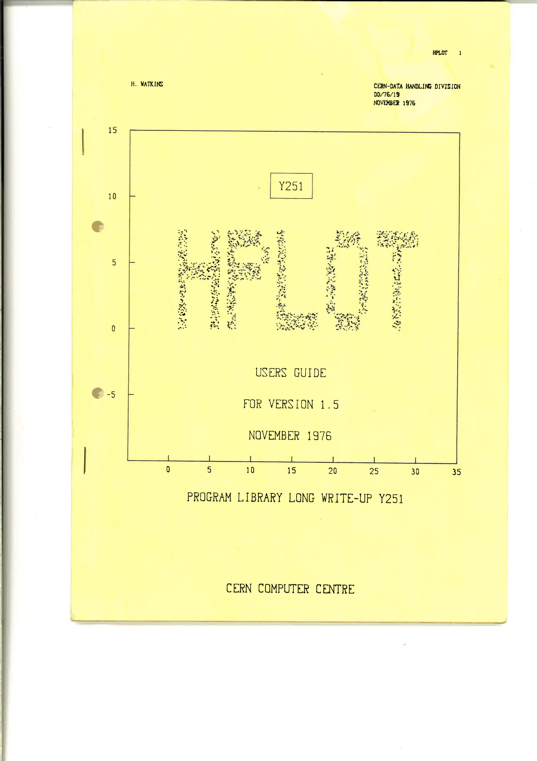
\includegraphics[width=0.2\textwidth]{hplot.png}
        ~~~~~
        
\includegraphics[width=0.2\textwidth]{htv.png}
        ~~~~~~~~~~~~~
        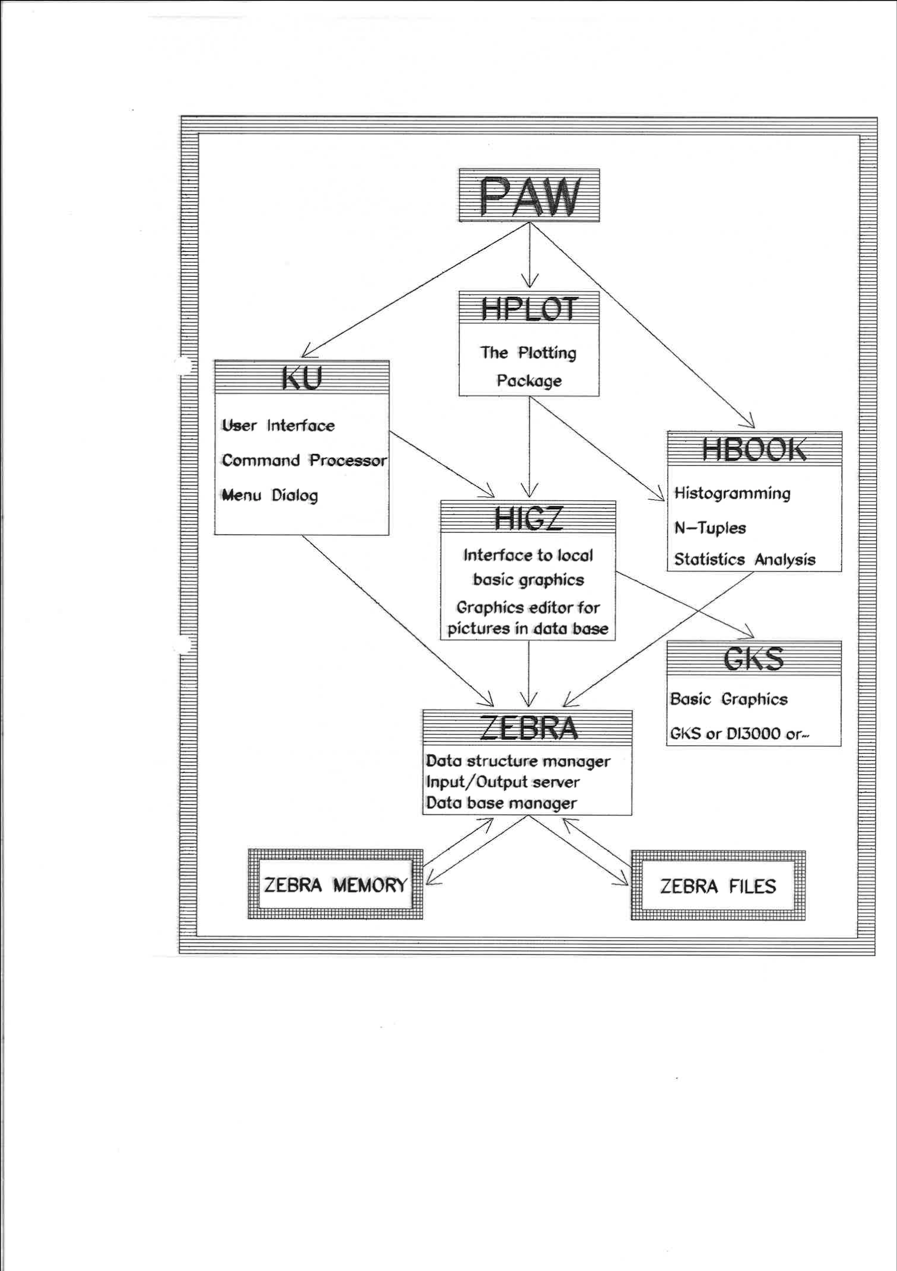
\includegraphics[width=0.2\textwidth]{paw-2.png}
        
\includegraphics[width=0.2\textwidth]{paw-1.png}

    HPLOT: $\approx$mid 70s ~~~~HTV: $\approx$early 80s~~~~~~~~~~~~~~~~~~~~~~~~~~~~~~~PAW: $\approx$1985
    \end{figure}
    \vspace{5mm}
    For a nice presentation on ROOT history and development take a look at \myhref{https://indico.cern.ch/event/667648/}{this CERN Data Science Seminar talk} by \textbf{Rene Brun} (includes also a recording).
%\begin{columns}
    %\begin{column}{0.6\textwidth}
    %\end{column}
    %\begin{column}{0.4\textwidth}
    %\begin{figure}
        %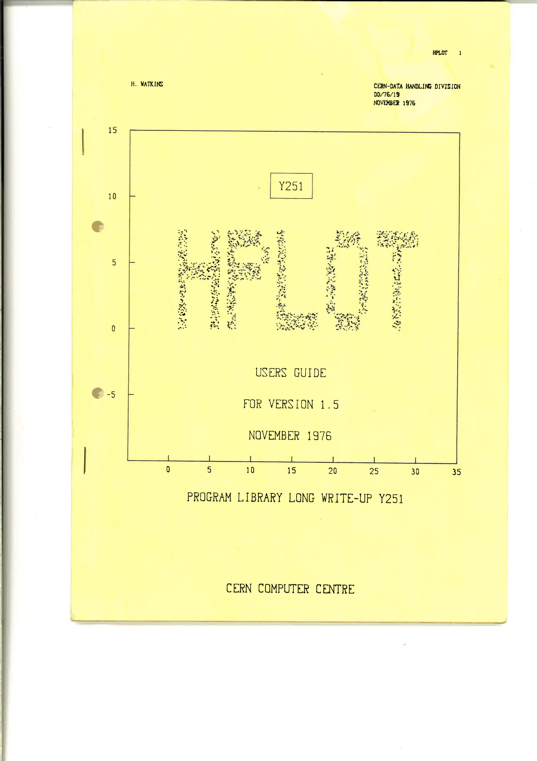
\includegraphics[width=0.4\textwidth]{hplot.png}
        %
\includegraphics[width=0.4\textwidth]{htv.png}
        %
\includegraphics[width=0.4\textwidth]{paw-1.png}
        %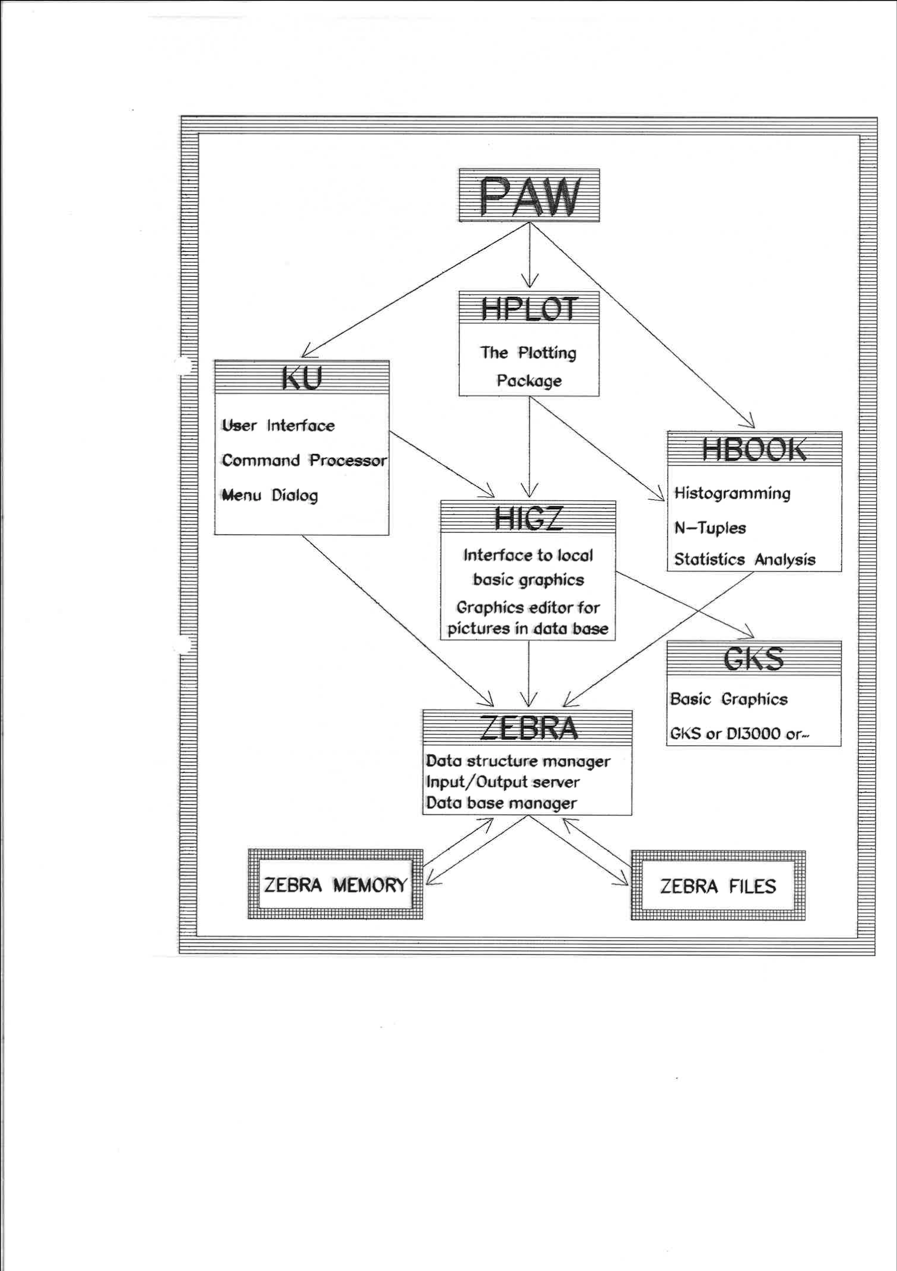
\includegraphics[width=0.4\textwidth]{paw-2.png}
    %\end{figure}
    %\end{column}
%\end{columns}
\end{frame}

\begin{frame}{ROOT in a nutshell}
ROOT can be seen as a collection of building blocks, like:
\begin{itemize}
    \item \textbf{Data analysis: histograms, graphs, functions}
    \item \textbf{I/O: row-wise, column-wise} storage of any C++ object
    \item \textbf{Statistical tools} (RooFit/RooStats): rich modeling and statistical inference
    \item Math: \textbf{non-trivial functions} (e.g. Erf, Bessel), optimized math functions
    \item \textbf{C++ interpretation}: full language compliance
    \item \textbf{Multivariate Analysis} (TMVA): e.g. Boosted decision trees, neural networks
    \item \textbf{Advanced graphics} (2D, 3D, event display)
    \item \textbf{Declarative Analysis}: RDataFrame
    \item And more: HTTP server, JavaScript visualization
\end{itemize}
\end{frame}


\begin{frame}{ROOT Application Domains}
    \myfigure{1.0}{root_domains.png}
\end{frame}

\begin{frame}{Resources}
\begin{itemize}
    \item ROOT website: \myhref{https://root.cern/}{https://root.cern/}
    \item Training: \myhref{https://github.com/root-project/training}{https://github.com/root-project/training}
    \item More material: \myhref{https://root.cern/get_started/}{https://root.cern/get\_started/}
    \begin{itemize}
        \item Includes a booklet for beginners: the \textbf{"ROOT primer"}
    \end{itemize}
    \item Reference guide: \myhref{https://root.cern/doc/master/index.html}{https://root.cern/doc/master/index.html}
    \item Forum: \myhref{https://root-forum.cern.ch/}{https://root-forum.cern.ch/}
    \item Tutorials: \myhref{https://root.cern/doc/master/group__Tutorials.html}{on the ROOT website}
\end{itemize}
    \vspace{3mm}
I encourage you to install ROOT yourself, just follow the \myhref{https://root.cern/install/}{install instructions} on the ROOT website!
    \begin{itemize}
        \item It is easiest if you have an un-to-date \textbf{macOS} or \textbf{Linux OS}
        \item On Windows, we recommend the \textbf{Windows subsystem for Linux} (\myhref{https://docs.microsoft.com/en-us/windows/wsl/about}{WSL})
    \end{itemize}
    \vspace{3mm}
    If you find any bugs please help us by opening a \myhref{https://github.com/root-project/root/issues}{GitHub issue}!
\end{frame}

\section{The different ways to use ROOT}

\begin{frame}{Ways to use ROOT}
\begin{itemize}
    \item The ROOT C++ command line interpreter
    \item C++ ROOT macros
    \item Compiled C++ using ROOT as a library
    \item As a library in Python code (\textbf{PyROOT})
\end{itemize}
\end{frame}


\begin{frame}[fragile]{The ROOT C++ interpreter}
By typing \texttt{root} in a terminal, you can fire up the ROOT C++ interpreter and execute arbitrary C++ statements
\begin{myterminal}
> root
root [0] int x = 4
(int) 4
root [1] int y = 5
(int) 5
root [2] x + y
(int) 9
root [3]
\end{myterminal}
\end{frame}

\begin{frame}[fragile]{Special commands in the ROOT C++ interpreter}
Special commands that are not C++ can be typed into the prompt, they start with a ".":
    \begin{myterminal}
root [0] .<command>
    \end{myterminal}
For example:
    \begin{itemize}
        \item To quit ROOT, use \textbf{.q}
        \item To issue a shell command, use \textbf{.! <OS command>}
        \item \textbf{.help} or \textbf{.?} gives the full list
    \end{itemize}
\end{frame}

\begin{frame}[fragile]{ROOT macros}
    Put a function with the same name as file in a \textbf{.C} file, for example \textbf{myMacro.C}:
\begin{cppcell}
void myMacro() {
   std::cout << "Hello World!" << std::endl;
}
\end{cppcell}
You can now run the code when starting the ROOT session:
\begin{myterminal}
> root myMacro.C
\end{myterminal}
Or you can run in from within a session:
\begin{myterminal}
> root
root [0] .x myMacro.C
\end{myterminal}
Or you can load it and run the function later:
\begin{myterminal}
root [0] .L myMacro.C
root [1] myMacro();
\end{myterminal}
\end{frame}

\begin{frame}[fragile]{Compiled C++ using ROOT as a library}
If you have a \textbf{main} function in the file, you can also compile the code with g++ for example:
\begin{cppcell}
void myMacro() {
   std::cout << "Hello World!" << std::endl;
}

int main() {
    myMacro();
}
\end{cppcell}
In the compilation command, you need to add the ROOT compiler flags:
\begin{myterminal}
> g++ -o myMacro myMacro.C `root-config --cflags --libs`
\end{myterminal}
You can now run your code like any other executable in the shell:
\begin{myterminal}
> ./myMacro
\end{myterminal}
\end{frame}

\begin{frame}[fragile]{As a library in Python code (also in Jupyter notebooks)}
If you import ROOT in a Python session or Python script, you can access ROOT functionality via its Python bindings (more on this later)
    \begin{pycell}
import ROOT
    \end{pycell}
\begin{itemize}
    \item You can also use ROOT in Jupyter notebooks like this
    \item If you want to run a notebook in the cloud, take a look at the \myhref{https://swan.cern.ch}{SWAN analysis interface}
    \item There is also a C++ kernel for the notebooks that comes with ROOT
    \item Notebooks are a great way to share and explain code to colleagues!
    \item However, for a large analysis project, it is better to \textbf{organize your code in Python scrips and modules!}
    \begin{itemize}
        \item This makes your analysis more reproducible and more independent of the backend
    \end{itemize}
\end{itemize}
\end{frame}

\section{Histograms, Graphs and Functions}

\begin{frame}[fragile]{Histograms}

\begin{itemize}
    \item{A simple form of data reduction}
    \begin{itemize}
        \item{Can have billions of collisions, the Physics displayed in a few histograms}
        \item{It is like an empirical density estimator}
        \item{Possible to calculate momenta: mean, rms, skewness, kurtosis}
    \end{itemize}
    \item{Collect quantities in discrete categories, the bins}
\end{itemize}

\begin{columns}
    \begin{column}{0.7\textwidth}

\begin{itemize}
    \item{ROOT Provides a rich set of histograms}
    \begin{itemize}
        \item{In multiple dimensions: \texttt{TH\{1,2,3\}} classes + \texttt{THN}}
        \item{Holding different precision types}
        \begin{itemize}
            \item{\texttt{TH1D} is a one-dim histogram holding doubles}
            \item{Have also:\\ \texttt{TH\{1,2,3\}F} (float), \texttt{I} (int32), \texttt{S} (int16), \texttt{C} (int8)}
        \end{itemize}
    \end{itemize}
\end{itemize}

\end{column}

    \begin{column}{0.3\textwidth}
        \myfigure{1.00}{CMS-HIG-12-028_Figure_003.pdf}
    \end{column}
\end{columns}

\end{frame}

\begin{frame}[fragile]{My First Histogram}

    \vspace{4mm}

    \begin{myterminal}
root [0] TH1D h("myHist", "myTitle", 64, -4.0, 4.0)
root [1] h.FillRandom("gaus")
root [2] h.Draw()
    \end{myterminal}

    \myfigure{0.6}{figure-001.pdf}

\end{frame}

\begin{frame}[fragile]{My First Histogram (in a notebook)}

    \textit{Note}| that in \textit{Jupyter notebooks} (also in \textit{SWAN}), the figure is not shown directly. You have to:
    \vspace{5mm}

    \begin{enumerate}
        \item Either call \texttt{gPad->Draw()} at the end:

              \begin{cppcell}
TH1D h("myHist", "myTitle", 64, -4.0, 4.0)
h.Draw()
gPad->Draw()
              \end{cppcell}

        \item Or you can create a TCanvas and draw it:

              \begin{cppcell}
TCanvas c1;
TH1D h("myHist", "myTitle", 64, -4.0, 4.0);
h.Draw();
c1.Draw();
              \end{cppcell}

    \end{enumerate}

\end{frame}

\begin{frame}{Functions}

\begin{itemize}
    \item{Mathematical functions are represented by the \textbf{TF1} class}
    \item{They have names, formulas, line properties, can be evaluated as well as their integrals and derivatives}
    \begin{itemize}
        \item{Numerical techniques for generic cases}
        \item{Automatic differentiation can be used for derivatives}
    \end{itemize}
\end{itemize}

\begin{columns}
    \begin{column}{0.6\textwidth}
        \vspace{0.5cm}
\begin{center}
    {\footnotesize
    \begin{tabular}{ |l|p{5.0cm}| }
 \hline
        \rowcolor{myblue} \textbf{\textcolor{white}{Option}} & \textbf{\textcolor{white}{Description}} \\
 \hline
 "SAME" & superimpose on top of existing picture \\
 \hline
 "L" & connect all computed points with a straight line \\
 \hline
 "C" & connect all computed points with a straight curve \\
 \hline
 "FC" & draw a fill area below a smooth curve \\
 \hline
\end{tabular}
    }
\end{center}
\begin{center}
    {\footnotesize From the \myhref{https://root.cern.ch/doc/master/classTGraphPainter.html}{TGraphPainter documentation}.}
\end{center}
\end{column}

    \begin{column}{0.4\textwidth}

% from https://tex.stackexchange.com/questions/270543/draw-a-graph-in-latex-with-tikz
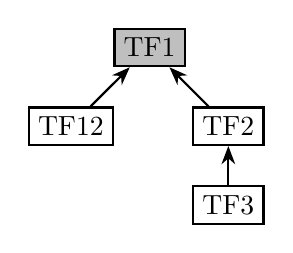
\begin{tikzpicture}
\begin{scope}[every node/.style={rectangle,thick,draw,fill=gray!50}]
    \node (TF1) at (1,2) {TF1};
\end{scope}
\begin{scope}[every node/.style={rectangle,thick,draw}]
    \node (TF12) at (0,1) {TF12};
    \node (TF2) at (2,1) {TF2};
    \node (TF3) at (2,0) {TF3};
\end{scope}

\begin{scope}[>={Stealth[black]},
              every node/.style={fill=white,circle},
              every edge/.style={draw=black,thick}]
    \path [->] (TF12) edge (TF1);
    \path [->] (TF2) edge (TF1);
    \path [->] (TF3) edge (TF2);
\end{scope}
\end{tikzpicture}

    \end{column}

\end{columns}

\end{frame}

\begin{frame}{Functions}

    Can describe functions as:

    \begin{itemize}
        \item Mathematical formulas (written as strings)
        \item C++ functions/functors/lambdas
              \begin{itemize} \item Implement your highly performant custom function \end{itemize}
        \item Python functions
              \begin{itemize} \item Fast prototyping on the Python side \end{itemize}
        \item With and without parameters
              \begin{itemize} \item Crucial for fits and parameter estimation \end{itemize}
    \end{itemize}


\end{frame}

\begin{frame}[fragile]{ROOT as a Function Plotter}

    The class TF1 represents one-dimensional functions (e.g., $f(x)$):

    \begin{myterminal}
root [0] TF1 f1("f1","sin(x)/x",0.,10.); // name, formula, min, max
root [1] f1.Draw();
    \end{myterminal}

    %\vspace{10mm}
    \begin{columns}
        \begin{column}{0.7\textwidth}

            An extended version of this example is the definition of a function
            with parameters:

            \begin{myterminal}
root [2] TF1 f2("f2","[0]*sin([1]*x)/x",0.,10.);
root [3] f2.SetParameters(1,1);
root [4] f2.Draw();
            \end{myterminal}
        \end{column}

        \begin{column}{0.3\textwidth}
            \myfigure{1.2}{figure-002.pdf}
        \end{column}
    \end{columns}

\end{frame}

\begin{frame}[fragile]{Another example}
    \begin{myterminal}
root [0] TH1D h("myHist", "myTitle", 64, -4, 4)
root [1] h.FillRandom("gaus")
root [2] h.Draw()
root [3] TF1 f("g", "gaus", -8, 8)
root [4] f.SetParameters(250, 0, 1)
root [5] f.Draw("Same")
    \end{myterminal}

    \myfigure{0.45}{figure-003.pdf}
\end{frame}

\begin{frame}{Graphs}
    \begin{columns}
        \begin{column}{0.5\textwidth}
            \begin{enumerate}
                \item Display points and errors
                \item Not possible to calculate momenta
                \item Not a data reduction mechanism
                \item \textbf{Fundamental to display trends}
                \item Focus on TGraph and TGraphErrors classes in this course
            \end{enumerate}
        \end{column}
        \begin{column}{0.5\textwidth}
            \myfigure{1.00}{Figure_005-a.pdf}
            \begin{center}
                {\small From \myhref{https://cds.cern.ch/record/2292159/}{CMS-PAS-HIG-17-019}.}
            \end{center}
        \end{column}
    \end{columns}
\end{frame}

\begin{frame}[fragile]{My first graph}


    \begin{myterminal}
root [0] TGraph g;
root [1] for (auto i : {0,1,2,3,4}) g.SetPoint(i,i,i*i)
root [2] g.Draw("APL")
    \end{myterminal}

    \myfigure{0.45}{figure-004.pdf}

\end{frame}

\begin{frame}[fragile]{Styling your graph}

    \begin{columns}
        \begin{column}{0.57\textwidth}

            \begin{myterminal}
g.SetMarkerStyle(kFullTriangleUp);
g.SetMarkerSize(3);
g.SetMarkerColor(kAzure);
g.SetLineColor(kRed - 2);
g.SetLineWidth(2);
g.SetLineStyle(3);
g.SetTitle("My Graph;The X;My Y");
gPad->SetGrid();
auto txt = "#color[804]{#mu {}^{40}_{20}Ca}";
TLatex l(.2, 10, txt);
l.Draw();
gPad->SetLogy();
            \end{myterminal}

        \end{column}
        \begin{column}{0.43\textwidth}
            \myfigure{1.1}{figure-005.pdf}
        \end{column}
    \end{columns}
    See also the \myhref{https://root.cern.ch/doc/master/classTAttMarker.html}{TAttMarker documentation} for details on the marker styles like \texttt{kFullTriangleUp} used in this example.

\end{frame}

%\begin{frame}[fragile]{The Marker Styles}
%\end{frame}

\begin{frame}[fragile]{The Color Wheel}
    \myfigure{0.5}{pict1_TColorWheel_001.png}
    From the \myhref{https://root.cern.ch/doc/master/classTColor.html}{TColor documentation}.
\end{frame}

\begin{frame}[fragile]{Drawing Options Documentation}
\begin{itemize}
    \item See the documentation of the \myhref{https://root.cern/doc/master/classTHistPainter.html}{THistPainterClass} for \textbf{histogram} drawing options
    \begin{figure}
        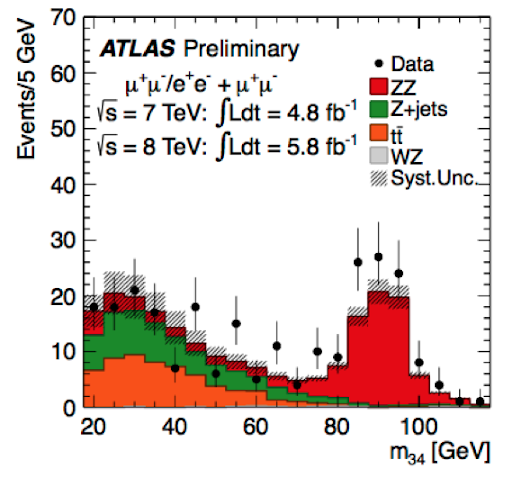
\includegraphics[width=0.2\textwidth]{hist-painter-1.png}
        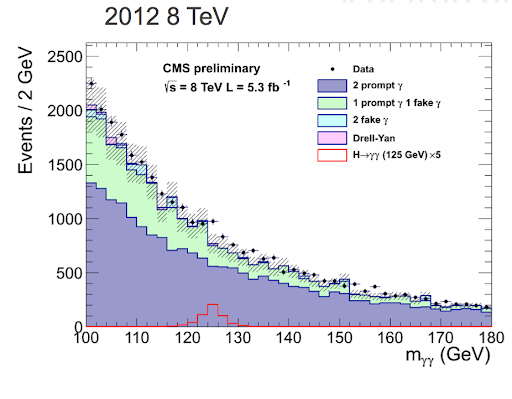
\includegraphics[width=0.28\textwidth]{hist-painter-2.png}
        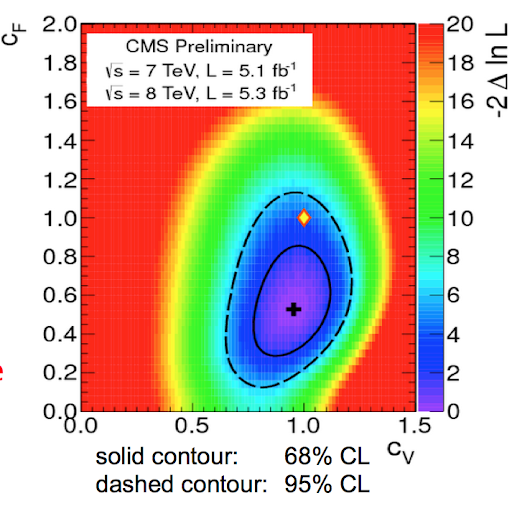
\includegraphics[width=0.2\textwidth]{hist-painter-3.png}
    \end{figure}
\item See the documentation of \myhref{https://root.cern/doc/master/classTGraphPainter.html}{TGraphPainter} for the \textbf{graph} drawing options
    \begin{figure}
        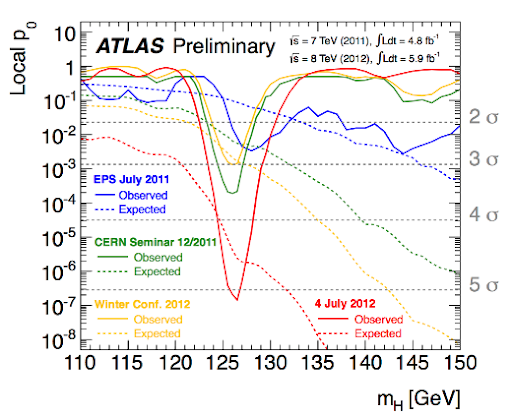
\includegraphics[width=0.25\textwidth]{graph-painter-1.png}
        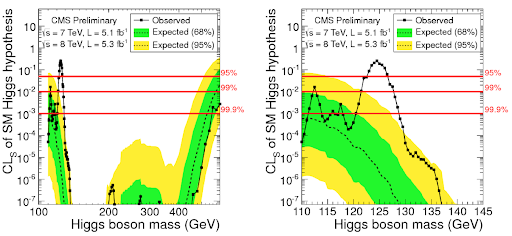
\includegraphics[width=0.43\textwidth]{graph-painter-2.png}
    \end{figure}
\end{itemize}
\end{frame}

\begin{frame}[fragile]{Example: stacked histograms}

In high energy physics, we often plot stacked histograms, for example to show the contributions of different processes. This can be doe with the \myhref{https://root.cern.ch/doc/master/classTHStack.html}{THStack}.
\vspace{3mm}

    \begin{columns}
        \begin{column}{0.57\textwidth}

            \begin{myterminaltiny}
TF1 f1{"f1", "gaus", -4.0, 4.0};

TH1D h1("h1", "x", 64, -4.0, 4.0);
TH1D h2("h2", "x", 64, -4.0, 4.0);
TH1D h3("h3", "x", 64, -4.0, 4.0);

THStack hs("hs","");
hs.SetTitle(";x;Events");

std::vector<TH1D*> histos{&h1, &h2, &h3};
std::vector<int> colors{46, 30, 38};

for(int i = 0; i < histos.size(); ++i) {
    TH1D & h = *histos[i];
    f1.SetParameters(1.0, i - 1, 1.0);
    h.FillRandom("f1", 100000);
    h.SetFillColor(colors[i]);
    hs.Add(&h);
}

hs.Draw();
            \end{myterminaltiny}

        \end{column}
        \begin{column}{0.43\textwidth}
            \myfigure{1.1}{figure-007.pdf}
        \end{column}
    \end{columns}

\end{frame}

\section{PyROOT: The ROOT Python Bindings}

\begin{frame}{PyROOT}
    \begin{itemize}
        \item Python bindings for ROOT
        \item Access all the ROOT C++ functionality from Python
              \begin{itemize} \item Benefit from C++ performance \end{itemize}
        \item Dynamic, automatic
        \item "Pythonizations" for specific cases
    \end{itemize}
    \vspace{5mm}
    In Python, you have also other great scientific and HEP-specific libraries that you \textbf{should also consider when they are the right tool for the job}!
    \begin{itemize}
        \item For example NumPy, Pandas, PyTorch, and Jax
        \item PyROOT is increasingly compatible with standard Python data structures like NumPy arrays
    \end{itemize}
\end{frame}

\begin{frame}{PyROOT spinoff: cppyy}
\begin{columns}
    \begin{column}{0.6\textwidth}
       \begin{itemize}
           \item{ROOTs technology to generate Python bindings automatically from C++ became an acclaimed standalong project: \textbf{cppyy}}
           \item{Prime example for how ROOT does cutting-edge R \& D also on the compiler and interpreter level}
       \end{itemize}
    \end{column}
    \begin{column}{0.4\textwidth}
        \myfigure{1.0}{cpp_weekly_cppyy.jpg}
        \textit{\myhref{https://www.youtube.com/watch?v=TL83P77vZ1k&t=153s}{Video on cppyy} in the C++ weekly channel.}
    \end{column}
\end{columns}
\end{frame}

\begin{frame}[fragile]{Using PyROOT}
    Entry point to use ROOT from Python:
    \begin{pycell}
        import ROOT
    \end{pycell}
    All the ROOT classes you have learned so far can be accessed from Python:
    \begin{pycell}
ROOT.TH1F
ROOT.TGraph
...
    \end{pycell}
\end{frame}

\begin{frame}[fragile]{Example: C++ to Python}
    \begin{columns}
        \begin{column}{0.65\textwidth}
            \begin{block}{C++}
                \begin{myterminal}
> root
root [0] TH1F h("myHist", "myTitle", 64, -4, 4)
root [1] h.FillRandom("gaus")
root [2] h.Draw()
                \end{myterminal}
            \end{block}
            \begin{block}{Python}
                \begin{myterminal}
> python
>>> import ROOT
>>> h = ROOT.TH1F("myHist", "myTitle", 64, -4, 4)
>>> h.FillRandom("gaus")
>>> h.Draw()
                \end{myterminal}
            \end{block}
        \end{column}
        \begin{column}{0.35\textwidth}
            \myfigure{1.2}{figure-001.pdf}
            \textit{Note: you can also use individual imports:}
            \begin{myterminal}
>>> from ROOT import TH1F
            \end{myterminal}
        \end{column}
    \end{columns}
\end{frame}

\begin{frame}[fragile]{Writing new C++ functions in PyROOT}
\begin{columns}
    \begin{column}{0.5\textwidth}
        Using \texttt{ROOT.gInterpreter.Declare()}, you can also define \textbf{new C++ functions}!
        \begin{pycell}
ROOT.gInterpreter.Declare("""
void myAdd(double a, double b) {
    return a + b;
}
""")
        \end{pycell}
        They are now in the \texttt{ROOT} module:
        \begin{pycell}
print(ROOT.myAdd(1.0, 2.0))
        \end{pycell}
    \end{column}
    \begin{column}{0.5\textwidth}
        In a \textbf{Jupyter notebook}, you can also use the \texttt{\%\%cpp} magic command:
        \begin{cppcell}
\%%%cpp
void myAdd(double a, double b) {
    return a + b;
}
        \end{cppcell}
        \begin{pycell}
print(ROOT.myAdd(1.0, 2.0))
        \end{pycell}
    \end{column}
\end{columns}

    \vspace{4mm}
Now you can define performant C++ functions for example to:

\begin{itemize}
    \item define fit functions
    \item transform event data (more on this later)
\end{itemize}

\end{frame}


\section{Parameter Estimation and Fitting}

\begin{frame}[fragile]{What is Fitting?}
\begin{itemize}
    \item{Estimate parameters of a hypothetical distribution from the observed data distribution}
    \begin{itemize}
        \item{$y = f(x|\theta)$ is the fit model function}
    \end{itemize}
    \item{Find the best estimate of the parameters $\theta$ assuming $f(x|\theta)$}
    \item{Both Likelihood and Chi2 fitting are supported in ROOT}
\end{itemize}


\begin{columns}
    \begin{column}{0.37\textwidth}
        \myfigure{0.9}{CMS-HIG-12-028_Figure_003.pdf}
    \end{column}
    \begin{column}{0.63\textwidth}
    \begin{center}
        \textbf{\textit{Example}}: $\text{Higgs}\to \gamma\gamma$ spectrum
    \end{center}
        We can fit for:
        \begin{itemize}
            \item the expected number of Higgs events
            \item the Higgs mass
        \end{itemize}
    \end{column}
\end{columns}


\end{frame}

\begin{frame}[fragile]{Fitting in ROOT}

\begin{itemize}
    \item{\textcolor{myblue}{\textbf{Create first a parametric function object}}, \texttt{TF1}, which represents our model}
    \begin{itemize}
        \item{need to set the initial values of the function parameters.}
    \end{itemize}
    \item{\textcolor{myblue}{\textbf{Fit the data object}} (Histogram or Graph):}
    \begin{itemize}
        \item{Call the \texttt{Fit} method passing the function object}
        \item{various options are possible (see the \texttt{\myhref{https://root.cern.ch/doc/master/classTH1.html\#a63eb028df86bc86c8e20c989eb23fb2a}{TH1::Fit}} documentation)}
    \end{itemize}
    \item{\textcolor{myblue}{\textbf{Examine result}}:}
    \begin{itemize}
        \item{get parameter values, uncertainties, correlation}
        \item{get fit quality estimation}
    \end{itemize}
\item{The resulting fit function is also drawn automatically on top of the Histogram or the Graph when calling \texttt{TH1::Fit} or \texttt{TGraph::Fit}}
\end{itemize}

\end{frame}

\begin{frame}[fragile]{Fitting Histograms}

    \begin{columns}
        \begin{column}{0.67\textwidth}

            Create a histogram, h1, and we want to fit it:
            \begin{myterminal}
root [0] TH1D h1("myHist", "myTitle", 64, -4.0, 4.0);
root [1] h1.FillRandom("gaus");
root [2] TF1 f1("f1","gaus");
root [3] h1.Fit(&f1);
            \end{myterminal}
            \vspace{-3mm}
            \begin{myterminaltiny}
 FCN=27.2252 FROM MIGRAD    STATUS=CONVERGED      60 CALLS          61 TOTAL
                     EDM=1.12393e-07    STRATEGY= 1      ERROR MATRIX ACCURATE
  EXT PARAMETER                                   STEP         FIRST
  NO.   NAME      VALUE            ERROR          SIZE      DERIVATIVE
   1  Constant     7.98760e+01   3.22882e+00   6.64363e-03  -1.55477e-05
   2  Mean        -1.12183e-02   3.16223e-02   8.18642e-05  -1.49026e-02
   3  Sigma        9.73840e-01   2.44738e-02   1.69250e-05  -5.41154e-03
            \end{myterminaltiny}
            For displaying the fit parameters:
            \begin{myterminal}
root [4] gStyle->SetOptFit(1111);
            \end{myterminal}

        \end{column}
        \begin{column}{0.33\textwidth}
            \myfigure{1.15}{figure-006.pdf}
        \end{column}
    \end{columns}

\end{frame}

\begin{frame}[fragile]{Creating the Fit Function}
    How to create the parametric function object (\textbf{TF1}):
    \begin{itemize}
        \item We can write formula expressions using functions:
            \begin{myterminal}
TF1 f1("f1","[0]*TMath::Gaus(x,[1],[2])");
            \end{myterminal}
        \begin{itemize}
            \item we can use the available functions in ROOT library and stl
            \item \textbf{[0],[1],[2] indicate the parameters.}
            \item We could also use meaningful names, like [a],[mean],[sigma]
        \end{itemize}
        \item There are pre-defined functions
            \begin{myterminal}
TF1("f1","gaus");
            \end{myterminal}
        \item pre-defined functions available: \textit{gaus, expo, landau, breitwigner,crystal\_ball,pol\{0,1..,N\}, cheb\{0,1,...10\},xygaus,,bigaus}
        \begin{itemize}
            \item see full list in the documentation of \myhref{https://root.cern.ch/doc/master/classTH1.html\#a63eb028df86bc86c8e20c989eb23fb2a}{TH1::Fit()}, and also in the \myhref{https://root.cern.ch/doc/master/classTFormula.html\#FormulaFuncs}{TFormula documentation}
        \end{itemize}

    \end{itemize}
\end{frame}

\begin{frame}{RooFit: ROOT toolkit for complex fitting}
\begin{columns}
\begin{column}{0.7\textwidth}
    \begin{itemize}
        \item ROOT fitting can handle complicated functions...
        \begin{itemize}
            \item ...but requires much code when fitting complex models
        \end{itemize}
    \item \myhref{https://root.cern/manual/roofit/}{RooFit} provides functionality for building fitting models
        \begin{itemize}
            \item complex model building from standard components
        \begin{itemize}
            \item composition with addition product and convolution
        \end{itemize}
        \end{itemize}
        \item Fitting often requires \textbf{normalization} of PDFs
        \begin{itemize}
            \item not always trivial and RooFit does it automatically
        \end{itemize}
        \item RooFit provides also
        \begin{itemize}
            \item \textbf{MC data generation} from model
            \item advanced \textbf{visualization} of fitting results
            \item \textbf{simultaneous fit} to different data samples
            \item full model description for \textbf{reusability}
            \item \textbf{built-in optimization} for optimal computational performances
            \begin{itemize}
                \item necessary for acceptable performance in complex fits
            \end{itemize}
        \end{itemize}
    \end{itemize}
    {\small \textit{For more info, see the \myhref{https://root.cern/topical/\#roofit}{manual} or the RooFit \myhref{https://root.cern/get_started/courses/\#roofitroostats-tutorials}{courses}}}.
\end{column}
\begin{column}{0.3\textwidth}
    \myfigure{1.25}{figure-008.pdf}
\end{column}
\end{columns}
\end{frame}


\begin{frame}{Likelihood fits in HEP}
\vspace{-0.5cm}
\begin{columns}
\begin{column}{0.5\textwidth}
    \begin{figure}
        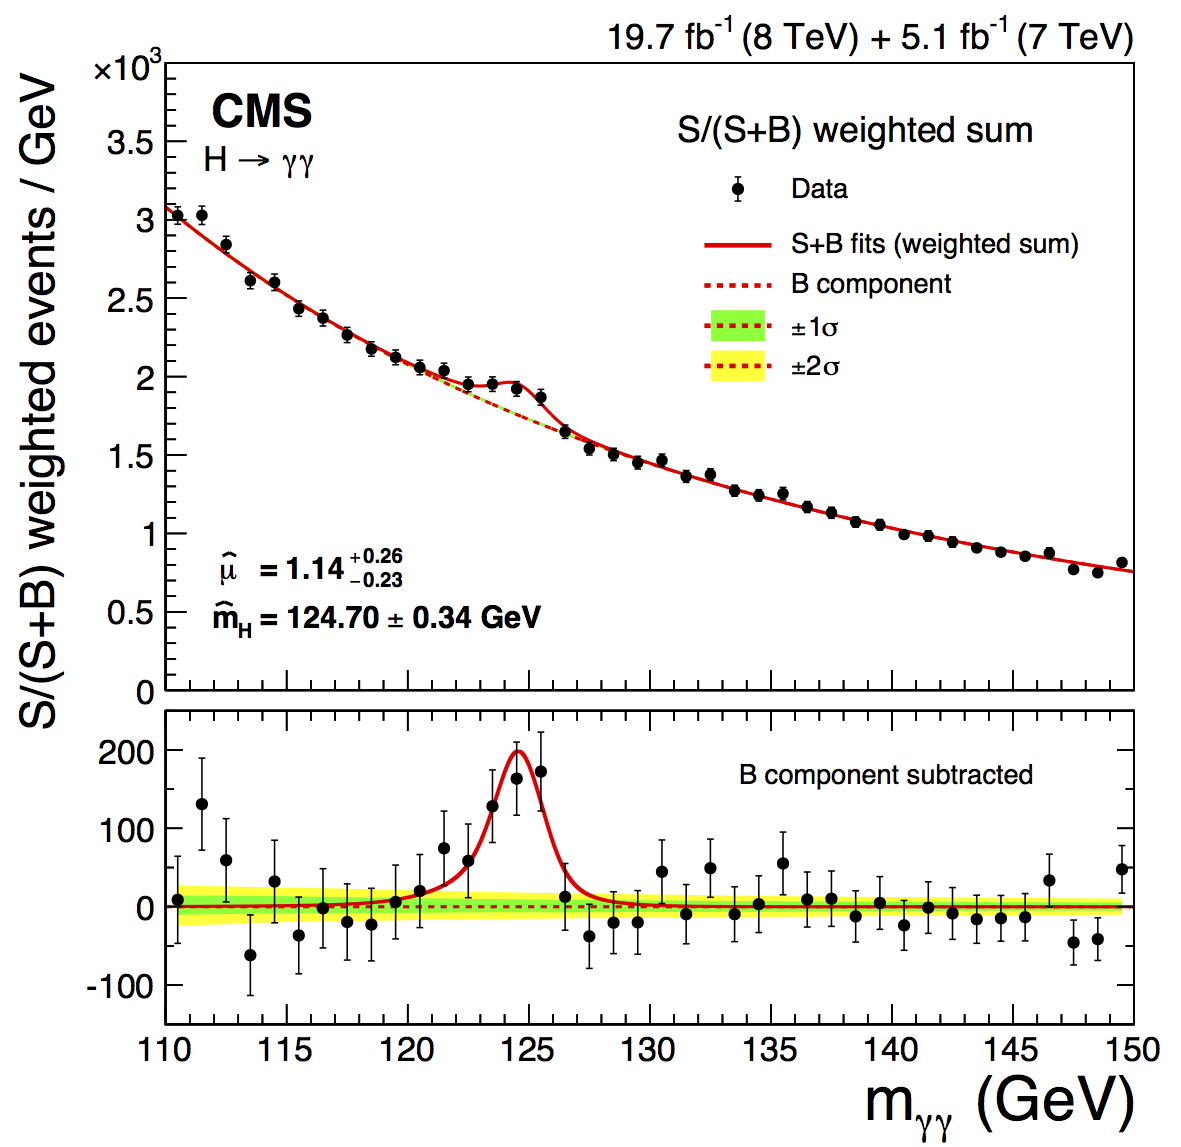
\includegraphics[width=0.7\textwidth]{gammagamma.png}
    \end{figure}
    %\vspace{-0.2cm}
    \textbf{Unbinned} likelihood fits
    \begin{itemize}
        \item often many events
        \item sums of PDFs of different types
    \end{itemize}
\end{column}
\begin{column}{0.5\textwidth}
    \begin{figure}
        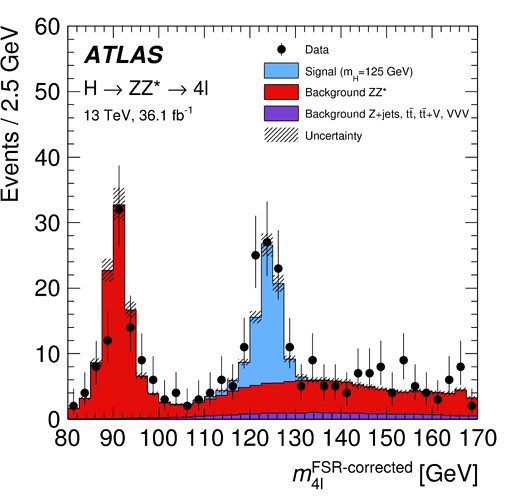
\includegraphics[width=0.7\textwidth]{fourleptons.png}
    \end{figure}
    %\vspace{-0.2cm}
    \textbf{Binned} likelihood fits
    \begin{itemize}
        \item often more params. than data points
        \item many per-bin nuisance parameters
    \end{itemize}
\end{column}
\end{columns}
\vspace{0.5cm}
    There are also often \textbf{combinations} of many binned and unbinned \textbf{channels}.
\end{frame}

\begin{frame}[fragile]{The need for an optimized data modeling library}
  \begin{itemize}
      \item Minimizing $NLL(\vec{x},\vec{\theta})$ with respect to $\vec{\theta}$ is done with the \texttt{Minuit} package, which uses numerical differentiation
    %\begin{itemize}
      %\item
    %\end{itemize}
    \item In num. diff, parameters are \textbf{one at a time} before re-evaluating the function
    \item $\Rightarrow$ idea: caching all intermediate results and re-evaluate only what is needed
  \end{itemize}
    \begin{figure}
        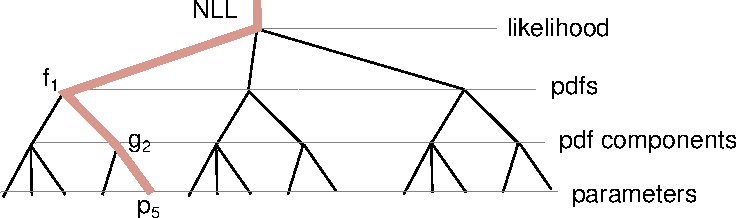
\includegraphics[width=0.5\textwidth]{graph.pdf}
    \end{figure}
  \begin{itemize}
      \item Drastically decreases the cost of gradient evaluation
  \end{itemize}

  \vspace{0.3cm}

    This is one of the central concepts in \textbf{RooFit}, enabling fits with 100s of pdfs and 1000s of parameters.
\end{frame}

\begin{frame}{How RooFit models are implemented}
\begin{columns}
\begin{column}{0.5\textwidth}
    \begin{itemize}
        \item Computation graph represented by C++ objects
        \item Objects are instances of classes that inherit from \texttt{RooAbsArg} class
        \item Top-level node is evaluated via chain of virtual function calls
        \item Has also some overhead from caching mentioned before
    \end{itemize}
\end{column}
\begin{column}{0.5\textwidth}
    \begin{figure}
        \includegraphics[width=1\textwidth]{model.png}
    \end{figure}
    \textit{\footnotesize The computation graph for a simple RooFit model.}
\end{column}
\end{columns}
    \vspace{0.5cm}
    Model definition by user is done usually at the level of declaring these C++ classes, although there are higher-level frameworks on top of RooFit.
\end{frame}

\begin{frame}[fragile]{RooFit example}
\begin{columns}
\begin{column}{0.5\textwidth}
Define variables (observables and params.):
\begin{myterminaltiny}
RooRealVar x{"x", "x", 0, 0, 10}; // observable

RooRealVar mu{"mu", "mu", 4, 0, 10};
RooRealVar sigma{"sigma", "sigma", 1, 0.01, 10};
RooRealVar c{"c", "c", -0.1, -10, -0.001};
\end{myterminaltiny}

Define pdf (here, Gaussian plus expo.):
\begin{myterminaltiny}
RooGaussian gauss{"gauss", "gauss", x, mu, sigma};
RooExponential expo{"expo", "expo", x, c};
RooAddPdf model{"model", "0.2 * gauss + 0.8 * expo",
                {gauss, expo}, {RooFit::RooConst(0.2)}};
\end{myterminaltiny}

Sample toy dataset:
\begin{myterminaltiny}
std::unique_ptr<RooDataSet> data{model.generate(x, 10000)};
\end{myterminaltiny}

Fit model to data with likelihood minim.:
\begin{myterminaltiny}
std::unique_ptr<RooFitResult> res{model.fitTo(*data)};
res->Print();
\end{myterminaltiny}
\end{column}
\begin{column}{0.5\textwidth}
Plotting
\begin{myterminaltiny}
RooPlot* frame = x.frame();
data->plotOn(frame);
model.plotOn(frame);
\end{myterminaltiny}
    \begin{figure}
        \includegraphics[width=1\textwidth]{figure-011.pdf}
    \end{figure}
\end{column}
\end{columns}
\end{frame}

\begin{frame}[fragile]{Normalization of pdfs}
Functions in RooFit can be evaluated with \texttt{getVal()}:
\begin{myterminal}
RooAbsReal &func = ...;
double val1 = func.getVal();
param.setVal(4.0);
double val2 = func.getVal(); // value updated automatically
\end{myterminal}

But the value of a pdf is \texttt{not well defined} without specifying which variables to normalize over!
\begin{myterminal}
RooAbsPdf &pdf = ...;
double val3 = pdf.getVal(); // not okay!
\end{myterminal}

You have to pass a "normalization set" to evaluate a pdf.
\begin{myterminal}
RooArgSet normSet{x1, x2};
double val4 = pdf.getVal(normSet);
\end{myterminal}
%Often, RooFit can figure out the normalization set from the context.
\end{frame}


\begin{frame}[fragile]{RooFit takes care of the integrals}
  \begin{columns}
    \begin{column}{0.5\textwidth}
        \begin{itemize}
            \item Normalization is done \textbf{automatically}
            \item Functions can be queried for analytical integral capabilities
            \begin{itemize}
                \item Similar interface for \textbf{sampling} as well
            \end{itemize}
            \item RooFit evaluates your likelihood with as little numerical integrals as possible
        \end{itemize}
        \textit{Conditional pdf example}:
        $$ p(x|y) = \frac{p(x,y)}{p(y)} = \frac{p(x,y)}{\int p(x,y)dx} $$
        \textit{Observable subdomain example}:
        $$ p(x|\text{subrange}) = p(x)\frac{\int_\text{full} p(x)dx}{\int_\text{subrange} p(x)dx} $$
    \end{column}
    \begin{column}{0.5\textwidth}
Define "model" as a pdf depending on $x$ and $y$ without caring about integrals:
\begin{myterminaltiny}
model = ...
\end{myterminaltiny}

NLL using p(x,y):
\begin{myterminaltiny}
nll1 = model.createNLL(dataXY);
\end{myterminaltiny}

NLL using p(x,y), restricted to defined \textbf{subrange}:
\begin{myterminaltiny}
nll2 = model.createNLL(dataXY, Range("subrange"));
\end{myterminaltiny}

\textbf{Conditional} NLL using p(x|y):
\begin{myterminaltiny}
nll3 = model.createNLL(dataXY, ConditionalObservables(y));
\end{myterminaltiny}
        \textit{\footnotesize More on this in the \myhref{https://root.cern/doc/master/rf303__conditional_8C.html}{RooFit conditional fit} tutorial.}
    \end{column}
  \end{columns}
\end{frame}

\begin{frame}[fragile]{RooFit Pythonizations}
\begin{columns}
    \begin{column}{0.5\textwidth}
Analyzers prefer Python:
    \begin{itemize}
        \item they want RooFit to be more \textbf{"pythonic"}
        \item they want interoperability with \textbf{NumPy} and \textbf{Pandas}
    \end{itemize}
\vspace{0.5cm}
We deliver now:

    \begin{itemize}
        \item \textbf{Pythonizations} of functions and classes, e.g., take builtin Python objects as arguments
    \item RooFit dataset classes interoperable with \textbf{NumPy} and \textbf{Pandas}
    \end{itemize}
\end{column}
    \begin{column}{0.5\textwidth}
    \vspace{-0.5cm}
    \begin{pycelltiny}
import ROOT

x = ROOT.RooRealVar("x", "x", -5, 5)
y = ROOT.RooRealVar("y", "y", -5, 5)
z = ROOT.RooRealVar("z", "z", -5, 5)

# Create background pdf poly(x)*poly(y)*poly(z)
px = ROOT.RooPolynomial("px", "px", x, [-0.1, 0.004])
py = ROOT.RooPolynomial("py", "py", y, [0.1, -0.004])
pz = ROOT.RooPolynomial("pz", "pz", z)
bkg = ROOT.RooProdPdf("bkg", "bkg", [px, py, pz])

data = bkg.generate((x, y, z), 20000)

df = data.to_pandas()
    \end{pycelltiny}
    \begin{myterminaltiny}
              x         y         z
0     -2.365318  4.625480  3.836555
1     -3.884152 -0.374631 -0.421798
2     -4.859738  3.288175 -1.899461
3     -2.307831  2.966785  0.909296
4     -1.253818  3.671417  3.595242
...         ...       ...       ...
19995 -0.433255  2.272059 -4.670626
19996  4.141638  1.365243 -0.250328
19997 -1.394192  0.792205 -1.647825
19998 -4.075001  0.499360  0.730352
19999  4.977131  1.158074 -0.679951

[20000 rows x 3 columns]
    \end{myterminaltiny}
\end{column}
\end{columns}
\end{frame}

\section{Reading and Writing Data}

\begin{frame}{The ROOT File}
\begin{itemize}
    \item With ROOT, you can write objects to files that are represented by \textbf{TFile} instances
    \item \texttt{.root} files are \textbf{binary} and can be compressed (transparently for the user)
    \item \textbf{TFiles are self-descriptive:}
    \begin{itemize}
        \item The information how to retrieve objects from a file is stored with the objects
    \end{itemize}
\end{itemize}

\begin{columns}
    \begin{column}{0.5\textwidth}
        \begin{itemize}
            \item ROOT files can contain simple tabluar data (aka. "n-tuples")
            \item It can also also contain \textbf{arbitrary custom C++ classes}
        \end{itemize}
\vspace{0.5cm}
{\footnotesize In case of future need: a \myhref{https://github.com/eguiraud/root_dictionaries_tutorial}{tutorial on how to save your custom classes}.}
    \end{column}
    \begin{column}{0.5\textwidth}
        \myfigure{1.1}{whats_in_aod_reco.png}
        \textit{Example of the custom classes saved in the CMS reconstruction output ROOT files.}
    \end{column}
\end{columns}

\end{frame}

\begin{frame}[fragile]{TFile in Action}

\begin{myterminal}
TFile f("myfile.root", "RECREATE");
\end{myterminal}

\begin{center}
    \begin{tabular}{ |l|p{6.5cm}| }
 \hline
        \rowcolor{myblue} \textbf{\textcolor{white}{Option}} & \textbf{\textcolor{white}{Description}} \\
 \hline
 NEW or CREATE & Create a new file and open it for writing. If the file already exists, it is not opened. \\
 \hline
 RECREATE & Create a new file. If the file already exists, it will be overwritten. \\
 \hline
 UPDATE & Open an existing file for writing. If no file exists, it is created. \\
 \hline
    READ & Open an existing file for reading (default) \\
 \hline
\end{tabular}
\end{center}
\end{frame}

\begin{frame}[fragile]{TFile in Action: Writing}

\begin{myterminal}
TFile f("file.root", "RECREATE");
TH1F h("h", "h", 64, 0.0, 8.0);
h.Write("h");
f.Close();
\end{myterminal}

\begin{itemize}
    \item Write to a file
    \item Close the file and make sure the operation succeeded
\end{itemize}

\begin{myterminal}
> rootls -l file.root
TH1F  Jun 24 15:02 2022 h  "h"
\end{myterminal}

\end{frame}

\begin{frame}[fragile]{TFile in Action: Reading}
%\begin{columns}
    %\begin{column}{0.5\textwidth}
        \begin{block}{C++}
            \begin{myterminal}
TFile f("file.root");
TH1F* h = f.Get<TH1F>("h");
h->Draw();
            \end{myterminal}
        \end{block}
    %\end{column}
    %\begin{column}{0.5\textwidth}
        \begin{block}{Python}
            \begin{myterminal}
import ROOT
f = ROOT.TFile("file.root")
f.h.Draw();
            \end{myterminal}
        \end{block}
        Get the histogram as an \textbf{attribute} of the TFile instance! Possible only in Python.
    %\end{column}
%\end{columns}
\end{frame}

\begin{frame}[fragile]{Listing TFile Content}
\begin{columns}
    \begin{column}{0.43\textwidth}
    \begin{itemize}
    \item \textbf{TBrowser}: interactive tool
    \begin{myterminal}
root [0] TBrowser tb
    \end{myterminal}
    \item \textbf{rootls} tool: list content
    \begin{myterminal}
> rootls file.root
    \end{myterminal}
    \item \textbf{TFile::ls()}: prints content
    \begin{myterminaltiny}
> root file.root
root [0]
Attaching file /mnt/file.root as _file0...
(TFile *) 0x562cbf485d50
root [1] _file0->ls()
TFile**		/mnt/file.root
 TFile*		/mnt/file.root
  KEY: TH1D	myHist;1	myTitle
root [2] .q
    \end{myterminaltiny}
    \begin{itemize}
        \item great for interactive usage
    \end{itemize}
    \end{itemize}
    \end{column}
    \begin{column}{0.57\textwidth}
    \myfigure{1.1}{tbrowser.png}
    \begin{center}
        {\small The new TBrowser in ROOT 6.26.}
    \end{center}
    \end{column}
\end{columns}
\vspace{2mm}
Note you can also open the file by passing it as a command line artument to \texttt{root}.
\end{frame}

\section{The ROOT Columnar Format and RDataFrame}

\begin{frame}{Columns and Rows}
    \begin{itemize}
        \item High Energy Physics: many statistically independent \textit{collision events}
        \item Create an event class, serialize and write out N instances into a file?
            \\ $\rightarrow$ No. Very inefficient!
        \item Organize the dataset in \textbf{columns}
    \end{itemize}
    \myfigure{0.8}{column-representation.png}
\end{frame}

\begin{frame}{The TTree}
    A columnar dataset in ROOT is represented by the \myhref{https://root.cern.ch/doc/master/classTTree.html}{TTree} class:
    \vspace{3mm}
    \begin{itemize}
        \item Also called \textit{tree} columns also called \textit{branches}
        \item Coloumns can contain different types
        \item \textbf{Supports any kind of object}
        \item One row per \textit{entry} (or, in collider physics, \textit{event})
    \end{itemize}
    \vspace{3mm}
    If just a \textbf{single number} per column is required, you can also use the simpler \myhref{https://root.cern.ch/doc/master/classTNtuple.html}{TNtuple} class.

    \vspace{3mm}

    {\color{darkgreen} A modern and simple way to interact with ROOT datasets is to use \myhref{https://root.cern/doc/master/classROOT_1_1RDataFrame.html}{RDataFrame}}.
    \vspace{3mm}
    \begin{itemize}
        \item Low-level interfaces to deal with datasets do exists
        \item There are many older scripts around that directly interact with TTrees
    \end{itemize}
\end{frame}

\begin{frame}[fragile]{RDataFrame: quick how-to}
    \begin{enumerate}
        \item \textbf{Build a dataframe} object by specifying your dataset
        \item Apply a series of \textcolor{red}{\textbf{transformations}} to your data
        \begin{itemize}
            \item \textbf{filter} (e.g., apply some cuts)
            \item define \textbf{new columns}
        \end{itemize}
    \item Apply \textcolor{blue}{\textbf{actions}} to the transformed data to produce results (e.g., filling a histogram)
    \end{enumerate}
\vspace{0.5cm}
See the \href{https://root.cern.ch/doc/master/group__tutorial__dataframe.html}{RDataFrame tutorials} for a comprehensive feature demo.
\end{frame}

\begin{frame}[fragile]{Simple Code Example (Python)}
    %\begin{cppcell}
%ROOT::RDataFrame rdf("tree", "file.root");
%auto hist = rdf.Filter("theta > 0").Histo1D("pt");
%hist->Draw();
    %\end{cppcell}
    \begin{pycell}
rdf = ROOT.RDataFrame("tree", "file.root")
hist = rdf.Filter("theta > 0").Histo1D("pt")
hist.Draw()
    \end{pycell}
    \begin{enumerate}
        \item Build RDataFrame
        \item Cut on \texttt{theta}
        \item Fill a histogram with $p_T$ and draw it
    \end{enumerate}
\end{frame}

\begin{frame}[fragile]{Filling multiple histograms}
    \begin{pycell}
h1 = rdf.Filter("theta > 0").Histo1D("pt")
h2 = rdf.Filter("theta < 0").Histo1D("pt")

h1.Draw()       // lazy evaluation: event loop is triggered here
h2.Draw("SAME") // no need to run event loop again!
    \end{pycell}
    \begin{itemize}
        \item Book all your actions upfront.
        \item The first time a result is accessed, RDataFrame will fill all booked results
        \item This \textbf{lazy evaluation} means that the {\color{red}{\textbf{iteration over events is only done once!}}}
        \item It is one of key ingredients for RDataFrames high performance
        \item Having a single event loop is \textit{particularly beneficial if you have to iterate over many files that don't fit in memory}
    \end{itemize}
\end{frame}

\begin{frame}[fragile]{More on histograms}
    \begin{pycell}
        h = rdf.Histo1D(("myName", "Title;x", 10, 0.0, 1.0), "x")
    \end{pycell}
    \begin{itemize}
        \item You can specify a model histogram with:
        \begin{itemize}
            \item a name and a title
            \item a predefined axis range and binning
        \end{itemize}
        \item Similar to the TH1 constructor you already know
        \item Here, the histogram is created with 10 bins ranging from 0 to 1, and the axis is labelled "x"
    \end{itemize}
\end{frame}

\begin{frame}[fragile]{Define a new column}
\begin{pycell}
mean = d.Filter("x > y")
        .Define("z", "sqrt(x*x + y*y)")
        .Mean("z");
\end{pycell}
\texttt{Define()} takes the name of the new column and its
expression. Later you can use the new column as if it
was present in your data.
\end{frame}

\begin{frame}[fragile]{Think of your analysis as a data flow}

\begin{columns}
    \begin{column}{0.6\textwidth}
\begin{pycell}
d2 = d.Filter("x > 0")
      .Define("z", "x*x + y*y")
# d2 is a new data-frame,
# a transformed version of d

# make multiple histograms out of it
hz = d2.Histo1D("z")
hx = d2.Histo1D("x")
\end{pycell}
You can store transformed data-frames in variables,
then use them as you would use an RDataFrame.
    \end{column}
    \begin{column}{0.4\textwidth}

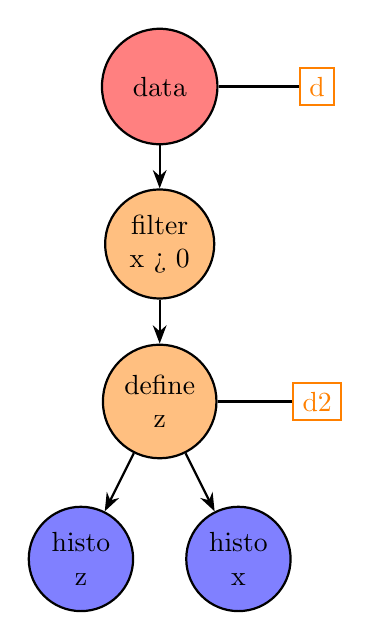
\begin{tikzpicture}
\begin{scope}[every node/.style={circle,thick,draw}]
    \node[align=center,fill=red!50] (data) at (1,6) {~~data~~};
    \node[align=center,fill=orange!50] (filter) at (1,4) {filter\\x > 0};
    \node[align=center,fill=orange!50] (define) at (1,2) {define\\z};
    \node[align=center,fill=blue!50] (histoz) at (0,0) {histo\\z};
    \node[align=center,fill=blue!50] (histox) at (2,0) {histo\\x};
\end{scope}
\begin{scope}[every node/.style={thick,draw}]
    \node[align=center,color=orange] (d) at (3,6) {d};
    \node[align=center,color=orange] (d2) at (3,2) {d2};
\end{scope}

\begin{scope}[>={Stealth[black]},
              every node/.style={fill=white,circle},
              every edge/.style={draw=black,thick}]
    \path [->] (data) edge (filter);
    \path [->] (filter) edge (define);
    \path [->] (define) edge (histoz);
    \path [->] (define) edge (histox);
\end{scope}

\begin{scope}[>={Stealth[black]},
              every node/.style={fill=white,circle},
              every edge/.style={draw=black,thick}]
    \path [-] (d) edge (data);
    \path [-] (d2) edge (define);
\end{scope}

\end{tikzpicture}

    \end{column}
\end{columns}

\end{frame}

\begin{frame}[fragile]{Cutflow reports}
\begin{pycell}
d.Filter("x > 0", "xcut")
 .Filter("y < 2", "ycut");

d.Report().Print();
\end{pycell}
When called on the main RDF object, \texttt{Report()} prints
statistics for all filters \textit{with a name}.
\begin{cellout}
xcut     : pass=49     all=100     --     49.000 %
ycut     : pass=22     all=49      --     44.898 %
\end{cellout}
\end{frame}

\begin{frame}[fragile]{Saving data to a file}
    \begin{pycell}
new_df = df.Filter("x > 0")
           .Define("z", "sqrt(x*x + y*y)")
           .Snapshot("tree", "newfile.root")
    \end{pycell}
We filter the data, add a new column, and then save
everything to file. No boilerplate code at all.
\end{frame}

\begin{frame}[fragile]{RDataFrame: declarative analysis}
    \begin{pycell}
df = ROOT.RDataFrame("treename", "file.root")
histo = df.Filter(is_good_entry, ["x","y"])
          .Histo1D("x")
    \end{pycell}
\begin{itemize}
    \item{full control over \textit{the analysis}}
    \item{no boilerplate}
    \item{common tasks are already implemented}
    \item{\textbf{parallelization is not trivial?}}
\end{itemize}
\end{frame}

\begin{frame}[fragile]{RDataFrame: parallelism}
\begin{pycell}
ROOT.EnableImplicitMT()
d = ROOT.RDataFrame("treename", "file.root")
h = d.Filter(is_good_entry, ["x","y"]).Histo1D("x")
\end{pycell}
\begin{itemize}
    \item{full control over \textit{the analysis}}
    \item{no boilerplate}
    \item{common tasks are already implemented}
    \item{parallelization is \textbf{automatic}!}
\end{itemize}
\end{frame}

\begin{frame}[fragile]{Defining new columns with C++}
You can always use C++ functions to define your new columns:
\begin{pycell}
ROOT.gInterpreter.Declare("""
auto calculateZ(float x, ROOT::VecOps::RVec<float>& y) {
    RVecF out;
    for(auto yi : y) {
        out.emplace_back(x * yi);
    }
    return out;
}
""")

rdf = rdf.Define("z", "calculateZ(x, y)")
\end{pycell}
Column \textbf{x} is of type \texttt{float}, \textbf{y} is a vector of floats, new column is vector of floats.

    This was just to demonstrate the principle. If you want to add \textbf{x + y} you better do:
\begin{pycell}
rdf = rdf.Define("z", "x + y")
\end{pycell}
\end{frame}

\begin{frame}[fragile]{ROOT's cutting-edge features: RDataFrame::Vary()}
    With the experimental \myhref{https://root.cern/doc/master/classROOT_1_1RDF_1_1RInterface.html\#a84d15369c945e4fe85e919224a0fc99f}{RDataFrame::Vary()}, you can efficiently declare variations of your analysis flow:
\begin{cppcell}
\%%%cpp
auto varyPt(double pt) {
    RVecD{pt*0.9, pt*1.1}; // returns a vector of variations
}
\end{cppcell}
\begin{pycell}
nominal_hx = df.Vary("pt", "varyPt", ("down", "up"))
      .Filter("pt > k")
      .Define("x", "someFunc", ("pt"))
      .Histo1D("x");
 
hx = ROOT.RDF.VariationsFor(nominal_hx)
hx["nominal"].Draw()
hx["pt:down"].Draw("SAME")
\end{pycell}
This streamlines greatly the treatment of \textbf{systematic variations}!
\end{frame}

\begin{frame}[fragile]{RDataFrame::Vary(): Example problem}
You have some analysis where you select events with exactly two electrons above some $p_T$ threshold:
\begin{pycell}
rdf = rdf.Filter("nElectron == 2")
// some logic to compute electron pair mass...

rdf = rdf.Define("ptCut", "10.0")
rdf = rdf.Filter("Electron_pt[0] > ptCut && Electron_pt[1] > ptCut")

h = rdf.Histo1D("Dielectron_mass")
h.Draw()
\end{pycell}
Your professor asks you:

\begin{center}
    "What if you change the $p_T$ cut? Produce all histos with different cut values."
\end{center}

\vspace{5mm}

$\Rightarrow$ \textbf{RDataFrame::Vary()} to the rescue!
\end{frame}

\begin{frame}[fragile]{RDataFrame::Vary(): A possible solution}
\begin{cppcell}
\%%%cpp
auto varyPtCut(double ptCut) {
    return RVecD{ptCut - 5, ptCut + 5};
}
\end{cppcell}
\begin{pycell}
rdf = rdf.Filter("nElectron == 2")
# some logic to compute electron pair mass...

rdf = rdf.Define("ptCut", "10.0")
rdf = rdf.Vary("ptCut", "varyPtCut(ptCut)", ("down", "up"))
rdf = rdf.Filter("Electron_pt[0] > ptCut && Electron_pt[1] > ptCut")

h = rdf.Histo1D("Dielectron_mass")
hvars = ROOT.RDF.Experimental.VariationsFor(h)

hvars["nominal"].Draw()
hvars["ptCut:down"].Draw("SAME")
hvars["ptCut:up"].Draw("SAME")
\end{pycell}
\end{frame}

\begin{frame}[fragile]{RDataFrame::Vary(): Example}
    \begin{columns}
        \begin{column}{0.5\textwidth}
        You are very happy with the solution:
        \vspace{3mm}
        \begin{itemize}
            \item Your whole analysis still runs in a single event loop
            \item Your new code with the three $p_T$ cut variations is \textbf{only 50 \% slower} than the original code
            \item Can you explain why that is?
        \end{itemize}
        \vspace{3mm}
        In particular for many variations, this sub-linear computation cost scaling is very important!
        \end{column}
        \begin{column}{0.5\textwidth}
            \myfigure{1.1}{vary.pdf}
        \end{column}
    \end{columns}
\end{frame}

\section{Wrapping up}

\begin{frame}{Conclusions}
\begin{itemize}
    \item ROOT is a \textbf{powerful toolkit} for the workflows specific to particle physics
    \begin{itemize}
        \item For analysis, \textbf{RooFit} and \textbf{RDataFrame} are useful in particular
    \end{itemize}
    \item There is lots of documentation on the internet, and if you are still stuck you will quickly get help on the very active \textbf{ROOT forum}!
    \item ROOT actively developed by the community for the \textbf{community}
    \begin{itemize}
        \item If you have ideas for improvements, don't hesitate to \textbf{engage} with the developers
    \end{itemize}
\item ROOT provides you performant algorithms written in \textbf{C++} that you can use in \textbf{Python} too, together with many other great Python libraries
\end{itemize}
    \vspace{5mm}
Thank you for you attention!

    %\vspace{5mm}

%We now move on to the hands-on tutorial, analyzing the Z boson with CMS Open Data.
\end{frame}

%\section{Hands-on tutorial session}

%\begin{frame}{Warm-up exercises}
    %To get familiar with the basics, we will first get started with some exercises from the official ROOT \myhref{https://github.com/root-project/training}{training repository}.
    %These exercises should take about 5 to 10 minutes each. Instructions can be found in the \textbf{readme.md} files in the linked directories:
    %\vspace{3mm}
    %\begin{enumerate}
        %\item The \myhref{https://github.com/root-project/training/tree/master/SummerStudentCourse/2022/Exercises/C\%2B\%2BInterpreter}{C++ interpreter introduction exercise}
        %\item The exercises on \myhref{https://github.com/root-project/training/tree/master/SummerStudentCourse/2022/Exercises/HistogramsGraphsFunctions}{histograms, graphs, and functions}
        %\item Parts of the \myhref{https://github.com/root-project/training/tree/master/SummerStudentCourse/2022/Exercises/Fitting}{fitting exercises}:
        %\begin{itemize}
            %\item We are only doing the \textbf{"Your First fit with ROOT"} and the \textbf{"Correlation of Parameters"} exercises today (the GUI fit panel is not covered in this lecture).
            %\item You are also not expected to go through the example notebooks today.
        %\end{itemize}
        %\item The \myhref{https://github.com/root-project/training/tree/master/SummerStudentCourse/2022/Exercises/PythonInterface}{PyROOT exercises}
        %\item The first \myhref{https://github.com/root-project/training/tree/master/SummerStudentCourse/2022/Exercises/WorkingWithColumnarData}{columnar data exercise}, called \textbf{"Analyse a Dataset"} in the \texttt{readme.md}.
        %\begin{itemize}
            %\item Instead of doing also the second part, we will do the more complex exercises on the next slides.
        %\end{itemize}
    %\end{enumerate}
    %\vspace{3mm}
    %The linked directories also contain \textbf{solutions} to the exercises.
%\end{frame}

%\begin{frame}{Advanced exercise}
    %\begin{itemize}
        %\item In this advanced exercise, you will write a little Z-Boson analysis based on the \texttt{DoubleElectron} CMS Open Data from \myhref{http://opendata.cern.ch/record/12367}{Run2012B}
            %and \myhref{http://opendata.cern.ch/record/12368}{Run2012C}
        %\item Please try to implement the following steps to \textbf{analyze the invariant mass} spectrum of electron pairs in the dataset:
    %\begin{enumerate}
        %\item Select events with exactly two electrons
        %\item Define \texttt{LorentzVectors} of the electrons
        %\item Calculate the invariant mass of the electron pairs
        %\item Fill a histogram
        %\item Fit the invariant mass Histogram to model the main resonance peak
        %\item Produce a nice plot with the data and the fit result
    %\end{enumerate}
%\item Can you model the peak accurately to \textbf{identify the mass of the Z boson}?
    %\end{itemize}
%\end{frame}

%\begin{frame}{Advanced exercise: hints}
%\begin{itemize}
    %\item TODO
%\end{itemize}
%\end{frame}

%\begin{frame}{Advanced exercise: possible solution and extra steps}
%\begin{columns}
    %\begin{column}{0.5\textwidth}
        %TODO.
    %\end{column}
    %\begin{column}{0.5\textwidth}
        %\myfigure{1.2}{zz.pdf}
            %{\small Quick solution fitting an exponential plus a Gaussian. Generated with only \textbf{30 lines of code}!}
    %\end{column}
%\end{columns}
%\end{frame}

\section{Backup - ROOT fitting details (if you're not using RooFit)}

\begin{frame}[fragile]{Building more Complex Functions}
\begin{itemize}
    \item{Any C++ object (functor) implementing}
    \begin{center}
        \texttt{double operator() (double *x, double *p)}
    \end{center}
            \begin{myterminal}
struct Function {
    double operator() (double *x, double *p){
        return p[0]*TMath::Gaus(x[0],p[1],p[2]);
    }
};
Function f;
TF1 f1("f1",f,xmin,xmax,npar);
            \end{myterminal}
    \item{Also a lambda function (with Cling and C++-11)}
            \begin{myterminal}
TF1 f1("f1",[](double *x, double *p){return p[0]*x[0];},0,10,1);
            \end{myterminal}
    \item{a lambda can be used also as a string expression, which will be JIT’ed by CLING}
            \begin{myterminal}
TF1 f1("f1","[](double *x, double *p){return p[0]*x[0];}",0,10,1);
            \end{myterminal}
\end{itemize}
\end{frame}

\begin{frame}[fragile]{Functionality provided by TFormula}
    \textcolor{myblue}{TFormula is based on Cling}. Additional functionality provided:
\begin{itemize}
    \item{better parameter definition}
    \begin{itemize}
        \item \texttt{TF1("f1",\textcolor{red}{"gaus(x, [Constant],[Mean],[Sigma])"});}
    \end{itemize}
    \item{function composition by concatenating expressions}
    \begin{itemize}
        \item \texttt{TF1 fs("\textcolor{blue}{sigma}",\textcolor{red}{"[0]*x+[1]"});}
        \item \texttt{TF1 f1("f1",\textcolor{red}{"gaus(x,[C],[Mean],\textcolor{blue}{sigma}(x,[A],[B])"});}
    \end{itemize}
    \item{normalized sum for component fitting}
    \begin{itemize}
        \item \texttt{TF1 model("model",\textcolor{red}{"NSUM(expo, gaus)"}, ...);}
    \end{itemize}
    \item{convolutions}
    \begin{itemize}
        \item \texttt{TF1 voigt("voigt", \textcolor{red}{"CONV(breitwiegner, gaus)"}, xmin, xmax);}
    \end{itemize}
    \item{can define vectorized functions for faster fitting and evaluation}
    \begin{itemize}
        \item see \myhref{https://root.cern.ch/doc/master/vectorizedFit_8C.html}{vectorizedFit} tutorial
    \end{itemize}
    \item{support for auto-differentiation (automatic generation of gradient and
Hessian)}
\end{itemize}
\end{frame}

\begin{frame}[fragile]{Fitting options}
\begin{itemize}
    \item{Likelihood fit for histograms}
    \begin{itemize}
        \item{option "L" for count histograms; \myterminalinline{h1->Fit("gaus","\emphinlisting{L}");}}
        \item{option "LW" in case of weighted counts. \myterminalinline{h1->Fit("gaus","\emphinlisting{LW}");}}
    \end{itemize}
    \item{Default is chi-square with observed errors (and skipping empty bins)}
    \begin{itemize}
        \item{option "P" for Pearson chi-square expected errors, and including empty bins \myterminalinline{h1->Fit("gaus","\emphinlisting{P}");}}
    \end{itemize}
\item{Use integral function of the function in bin \myterminalinline{h1->Fit("gaus","\emphlightinlisting{L} \emphinlisting{I}");}}
\item{Compute MINOS errors : option "E" \myterminalinline{h1->Fit("gaus","\emphlightinlisting{L} \emphinlisting{E}");}}
\end{itemize}
\end{frame}

\begin{frame}[fragile]{Some more Fitting Options}

\begin{columns}
\begin{column}{0.52\textwidth}
\begin{itemize}
    \item{Fitting in a Range \myterminalinline{h1->Fit("gaus","","",\emphinlisting{-1.5,1.5});}}
    \item{For doing several fits \myterminalinline{h1->Fit("expo","+","",2.,4);}}
    \item{Quiet / Verbose: option "Q"/"V" \myterminalinline{h1->Fit("gaus",\emphinlisting{"V"});}}
    \item{Avoid storing and drawing fit function (useful when fitting many times) \myterminalinline{h1->Fit("gaus","\emphlightinlisting{L} \emphinlisting{N 0}");}}
    \item{Save result of the fit, option "S"}
        \begin{myterminal}
auto result = h1->Fit("gaus","L S");
result->Print("V");
        \end{myterminal}
\end{itemize}
{\footnotesize All fitting options documented in reference guide or User Guide (Fitting Histogram chapter)}
\end{column}

\begin{column}{0.48\textwidth}
\myfigure{1.0}{figure-010.pdf}
\begin{center}
    {\footnotesize Example of ranged fit.}
\end{center}
\end{column}
\end{columns}

\end{frame}

\begin{frame}[fragile]{Parameter Errors}
Errors returned by the fit are computed from the second derivatives of the
log-likelihood function
\begin{itemize}
    \item{Assume the negative log-likelihood function is a parabola around minimum}
    \item{This is true asymptotically and in this case the parameter estimates are also normally distributed.}
    \item{The estimated correlation matrix is then:}
\end{itemize}
    \vspace{-1cm}
\begin{columns}
\begin{column}{0.57\textwidth}
        $$\hat{V}(\hat{\theta}) = \left[ \left(-\frac{\partial^2\text{ln}L(x;\theta)}{\partial^2\theta}\right)_{\theta=\hat{\theta}} \right]^{-1} = H^{-1}$$
\end{column}
\begin{column}{0.43\textwidth}
    \myfigure{1.00}{figure-009.pdf}
\end{column}
\end{columns}

\end{frame}

\end{document}
